\documentclass{standalone}

\usepackage{pgfplots}
\pgfplotsset{compat=newest}

\begin{document}
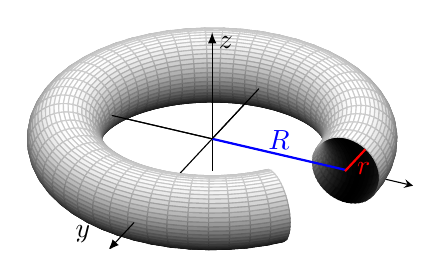
\begin{tikzpicture}
  \begin{axis}[
      axis equal image,
      axis lines=middle,
      xmax=18,zmax=5,
      ticks=none,
      clip bounding box=upper bound,
      colormap/blackwhite
    ]

    \addplot3[domain=0:360,y domain=0:320, samples=50,surf,z buffer=sort]
    ({(12 + 3 * cos(x)) * cos(y)} ,
    {(12 + 3 * cos(x)) * sin(y)},
    {3 * sin(x)});
    % use axis coordinate system to draw the radii
    \draw [thick,blue] (axis cs: 0,0,0) -- (axis cs: 12,0,0) node [midway,above=-2] {$R$};
    \draw [thick,red] (axis cs: 12,-0.2,0) -- (axis cs: 12,3.7,0) node [midway,below right=-3] {$r$};

    % use axis coordinate system to draw fake x, y and z axes
    \draw [-latex] (axis cs: 0,0,0) -- node [pos=0.9, xshift=0.5em]{$z$}(axis cs: 0,0,10);
    \draw [-latex] (axis cs: 0,-15,0) --
    node [pos=0.9, xshift=-1em, yshift=0.5em]{$y$}(axis cs: 0,-20,0);
    \draw (axis cs: 0,0,0) -- (axis cs: 0,9,0);
    \draw (axis cs: 0,0,0) -- (axis cs: -9,0,0);
  \end{axis}
\end{tikzpicture}
\end{document}
